\documentclass[10pt]{article}

\usepackage{fancyhdr}
\usepackage{extramarks}
\usepackage{amsmath}
\usepackage{amsthm}
\usepackage{amsfonts}
\usepackage{tikz}
\usepackage[plain]{algorithm}
\usepackage{algpseudocode}
\usepackage{ragged2e}
\usetikzlibrary{automata,positioning}
\usepackage{setspace}
\usepackage{etoolbox}
\usepackage{enumitem}
\usepackage{hyperref}
\hypersetup{colorlinks=true,allcolors=blue}
\usepackage{hypcap}
\usepackage{graphicx}    %for figure environment.
\usepackage{calc}
\usepackage{ifthen}
\usepackage{tikz}
\usepackage{longtable}
\usepackage{lipsum}
\usepackage{verbatim}
\usepackage{enumitem}
\setlist[enumerate]{itemsep=0mm}
\setlist[itemize]{itemsep=0mm}
\usepackage{pstricks-add}
\usepackage{pstricks}
\usepackage{rotating}
\usepackage{mathtools}


\makeatletter
\pretocmd{\@sect}{\singlespacing}{}{}
\pretocmd{\@ssect}{\singlespacing}{}{}
\apptocmd{\@sect}{\singlespacing}{}{}
\apptocmd{\@ssect}{\singlespacing}{}{}
\makeatother

%
% Basic Document Settings
%
\newcommand{\ts}{\textsuperscript}

%\begin{comment}
\topmargin=-0.45in
\evensidemargin=0in
\oddsidemargin=0in
\textwidth=6.5in
\textheight=9.0in
\headsep=0.25in
%\end{comment}

\linespread{1.1}

\pagestyle{fancy}
\lhead{\hmwkAuthorName}
\chead{\textbf{\hmwkClass : \hmwkTitle}}
\rhead{\hmwkAuthorNumber}
\lfoot{\lastxmark}
\cfoot{\thepage}

\renewcommand\headrulewidth{0.4pt}
\renewcommand\footrulewidth{0.4pt}

\setlength\parindent{0pt}

%
% Create Problem Sections
%


\setcounter{secnumdepth}{0}
\newcounter{partCounter}
\newcounter{homeworkProblemCounter}
\setcounter{homeworkProblemCounter}{1}
\nobreak\extramarks{Problem \arabic{homeworkProblemCounter}}{}\nobreak{}

%
% Homework Problem Environment
%
% This environment takes an optional argument. When given, it will adjust the
% problem counter. This is useful for when the problems given for your
% assignment aren't sequential. See the last 3 problems of this template for an
% example.
%


%
% Homework Details
%   - Title
%   - Due date
%   - Class
%   - Section/Time
%   - Instructor
%   - Author
%

\newcommand{\hmwkTitle}{Assignment 2\ \ }
\newcommand{\hmwkDueDate}{Sunday, November 12\ts{th}, 2017}
\newcommand{\hmwkClass}{CSC411}
\newcommand{\hmwkClassTime}{Section A}
\newcommand{\hmwkClassInstructor}{Steven Chuang}
\newcommand{\hmwkClassTeachingAssistant}{Natalia Mykhaylova}
\newcommand{\hmwkAuthorName}{Gokul K. Kaushik}
\newcommand{\hmwkAuthorNumber}{999878191}
\newcommand{\schoolmate}{\textsc{School-Mate }}

\newcommand\Tstrut{\rule{0pt}{2.6ex}}       % "top" strut
\newcommand\Bstrut{\rule[-0.9ex]{0pt}{0pt}} % "bottom" strut
\newcommand{\TBstrut}{\Tstrut\Bstrut} % top&bottom struts
%
% Title Page
%

\title{
    \vspace{2in}
    \textmd{\textbf{\hmwkClass:\ \hmwkTitle}}\\
    \vspace{0.1in}\small{Due\ on\ \hmwkDueDate}\\
    \vspace{3in}
    \vspace{0.1in}\large{Student Name: \textbf{\hmwkAuthorName} } \\
    \vspace{0.1in}\large{Student Number: \textbf{\hmwkAuthorNumber} } \\
}

%\author{\textbf{\hmwkAuthorName}}
%\textbf{\hmwkAuthorNumber\}
\date{}

\renewcommand{\part}[1]{\textbf{\large Part \Alph{partCounter}}\stepcounter{partCounter}\\}

%
% Various Helper Commands
%

% Useful for algorithms
\newcommand{\alg}[1]{\textsc{\bfseries \footnotesize #1}}

% For derivatives
\newcommand{\deriv}[1]{\frac{\mathrm{d}}{\mathrm{d}x} (#1)}

% For partial derivatives
\newcommand{\pderiv}[2]{\frac{\partial}{\partial #1} (#2)}

% Integral dx
\newcommand{\dx}{\mathrm{d}x}

% Alias for the Solution section header
\newcommand{\solution}{\textbf{\large Solution}}

% Probability commands: Expectation, Variance, Covariance, Bias
\newcommand{\E}{\mathrm{E}}
\newcommand{\Var}{\mathrm{Var}}
\newcommand{\Cov}{\mathrm{Cov}}
\newcommand{\Bias}{\mathrm{Bias}}
\renewcommand*\contentsname{Table of Contents}

\begin{document}
\maketitle
\pagebreak

\begin{center} \tableofcontents \end{center}
\pagebreak

\clearpage
\setcounter{page}{1}

\section{1 - Class Conditional Gaussians}
\subsection{1 - Using Bayes’ rule to derive an expression for $p(y = kx, \mu,\sigma)$}
\subsection{2 - Expression for the negative likelihood function (NLL)}
\subsection{3 - Partial Derivatives of the Likelihood}
\subsection{4 - Find the maximum likelihood estimates for $\mu$ and $\sigma$}


\section{2 - Handwritten Digit Classification}
\subsection{0 - Loading the data and Plotting the Feature Means}

The means (from 700 samples per digit) for each feature (64 features in total for an 8-by-8 pixel image) for 10 digits (digit 0 to digit 9) are plotted below: 

\begin{center}
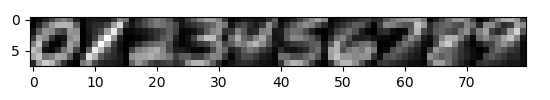
\includegraphics[scale=1]{averages.png}
\end{center}


\subsection{1 -  K-NN Classifier}
\subsection{2 -  Conditional Gaussian Classifier Training}
\subsection{3 -   Naive Bayes Classifier Training}
\subsection{4 -  Model Comparison}


\pagebreak


\end{document}


$
0.999999942522
\iffalse
\section{(Part 1) Learning Basics of Regression in Python}

\subsection{Describe and Summarize the data}
\label{sec:rangez}
\begin{itemize}
  \item 506 data samples
  \item 13 input (explanatory features) named:
  \begin{enumerate}
		\item  CRIM (range: 0.00632 - 88.9762 )
		\item  ZN (range: 0.0 - 100.0 )
		\item  INDUS (range: 0.46 - 27.74 )
		\item  CHAS (range: 0.0 - 1.0 ) which is binary as it only takes a value between 0.0 and 1.0 and nothing in between.
		\item  NOX (range: 0.385 - 0.871 )
		\item  RM (range: 3.561 - 8.78 )
		\item  AGE (range: 2.9 - 100.0 )
		\item  DIS (range: 1.1296 - 12.1265 )
		\item  RAD (range: 1.0 - 24.0 )
		\item  TAX (range: 187.0 - 711.0 )
		\item  PTRATIO (range: 12.6 - 22.0 )
		\item  B (range: 0.32 - 396.9 )
		\item  LSTAT (range: 1.73 - 37.97 )
	\end{enumerate}   
  \item Features consists of real and positive numbers
  \item Target name is MEDV, the median value of a house and it consists of real numbers (range: 5.0 - 50.0)
\end{itemize}


\subsection{Visualization}
This is a plot of every feature against the target where the feature and targets are on the x and y-axes of the Cartesian plane respectively. 

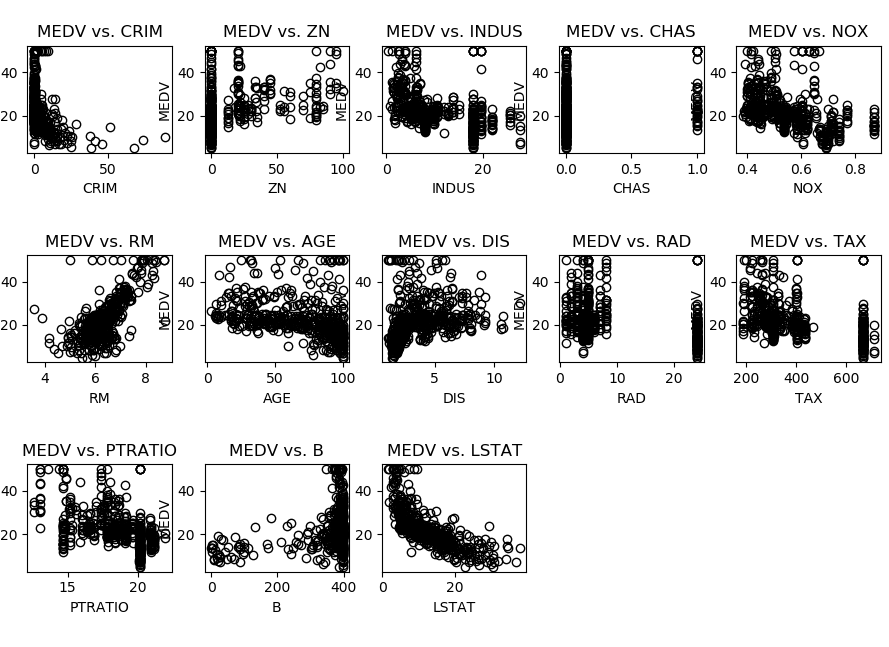
\includegraphics[scale=0.74]{plot.png}

\pagebreak

\subsection{Feature Weights}

\def\arraystretch{1.5}
\label{Housing Features}
\label{sec:hfs}
\begin{tabular}{llll}
\textbf{\#} & \textbf{Feature Name} & \textbf{Value} & \textbf{Description}                                                           \\ \hline
0           & Bias                  & 34.72315854    & \textbf{Not a feature - Bias Value}                                  \\ \hline
1           & CRIM                  & -0.1001396     & per capita crime rate by town                                                  \\ \hline
2           & ZN                    & 0.0411024      & proportion of residential land zoned for lots over 25,000 sq.ft.               \\ \hline
3           & INDUS                 & 0.02359639     & proportion of non-retail business acres per town                               \\ \hline
4           & CHAS                  & 2.74448198     & Charles River dummy variable (= 1 if tract bounds river; 0 otherwise)          \\ \hline
5           & NOX                   & -17.49103746   & nitric oxides concentration (parts per 10 million)                             \\ \hline
6           & RM                    & 4.16892358     & average number of rooms per dwelling                                           \\ \hline
7           & AGE                   & -0.01047614    & proportion of owner-occupied units built prior to 1940                         \\ \hline
8           & DIS                   & -1.4367399     & weighted distances to five Boston employment centres                           \\ \hline
9           & RAD                   & 0.29696781     & index of accessibility to radial highways                                      \\ \hline
10          & TAX                   & -0.01349442    & full-value property-tax rate per \$10,000                                      \\ \hline
11          & PTRATIO               & -0.93914748    & pupil-teacher ratio by town                                                    \\ \hline
12          & B                     & 0.00733658     & 1000(Bk - 0.63)\textasciicircum 2 where Bk is the proportion of blacks by town \\ \hline
13          & LSTAT                 & -0.45653296    & \% lower status of the population                                              \\ \hline
\\
\end{tabular}
\def\arraystretch{1}

INDUS, as the \hyperref[sec:hfs]{table} states, is the proportion of non-retail business acres per town. The weight associated with it is positive implying a positive correlation with the target (i.e. an increase or decrease in INDUS will result in an increase or decrease in the housing price respectively). 
\\ \\
However, 0.023 is a minuscule in magnitude and this means that a large change in INDUS will result in a small change in the housing price. Therefore, INDUS is a statistically insignificant explanatory variable. 
\\ \\
This makes sense as the non-retail business acres per town would is a secondary feature relative to: pollution, number of rooms, population status, and the Charles River. 

\subsection{Mean Squared Error Value}
The MSE obtained from the test set was \textbf{23.423}.

\subsection{Two Other Loss Functions}
Two other loss functions that were used are: 
\begin{enumerate}
\item \textbf{The Absolute Loss function}, $L_1$:

\[L_{1} = 
\sum_{i=1}^{N}
|y^{(i)} - \textbf{w}^T\textbf{x}^{(i)}|
\]

The loss function gave us an error of \textbf{3.722}. It was chosen as the $L_2$ loss function heavily penalizes outliers, whereas, the $L_1$ penalizes all samples equally. The huge difference between $L_2$'s 23.423 and $L_1$'s 3.722 (even squared is below 16) shows that there are a number of outlier points that $L_2$ has penalized. This outlier set could be anomalies that the loss function should not optimize for and $L_1$ tells us this.

\item \textbf{The Huber Loss function} $L_{\delta}$: 
\[
L_{\delta} = 
\begin{cases}
{\frac{1}{2}(y-f(x))^2} & {} \text{for }|y-f(x)|
\leq \delta
\\{\delta|y-f(x)| - \frac{1}{2}\delta^2} & \text{otherwise}\end{cases}
\]

This function gave us an error of \textbf{4.204}. It was chosen as it gives us the best of both $L_1$ and $L_2$. It heavily penalizes nearby points (using the square of the distance) and ignores distant outliers (by treating them as an $L_1$ loss). The point at which it switches between either case is determined by $\delta$, a user defined parameter. Using the standard value of $\delta = 1.35$, the error was obtained. It was closer to the $L_1$ loss rather than the $L_2$. This further justifies the existence of many outliers and shows there are far more consistently close samples. 


\end{enumerate}

\subsection{Most Significant Features}

The most significant features from the table by magnitude and logic are \textbf{in no order}:
\begin{itemize}
\item \textbf{CRIM (-0.10)}: The per capita \textbf{crime rate} has a negative correlation with the price. Crime is a deterrent to raising housing prices.
\item \textbf{CHAS (2.74)}: Houses along the \textbf{Charles River} are more expensive, which is plausible as they might be prime real-estate due to their view and access to the river. 
\item \textbf{NOX (-17)}: Housing prices should be \textbf{lower in polluted areas} and this remains true with the negative correlation in the MEDV vs NOX graph. However, the large weight value for pollution is probably due to its small magnitude as a feature (~0.4-~0.9).
\item \textbf{RM (4.16)}: Houses with \textbf{more rooms should be more expensive }and that remains the case. The number of rooms and the size of the house is generally what is listed in the housing flyers (important) and the weight confirms this. 
\item \textbf{LSTAT (-.45)}: Houses in neighbourhoods with \textbf{lower status would be cheaper}. The graph also shows a linear negative correlation between MEDV vs LSTAT. The low weight value is could be because of its high mean sample value.
\item \textbf{TAX (-.013)}: The higher the property tax, the less incentive for buyers to buy. Taxes has a large sample values (from 187 to 711). The weight associated with it might not accurately represent its importance.
\end{itemize} 

\textbf{Note}: The \hyperref[sec:hfs]{feature weights table}'s weights were taken as is based on the instructions of the assignment. Features have different \hyperref[sec:rangez]{value ranges}. Therefore, features with low value ranges, and are in reality good predictors, could have an exponentially higher weight to compensate for the low magnitude range. In order to have a less biased view, \textbf{feature scaling should be performed, after which, weights calculated}.

\pagebreak
\section{(Part 2) Locally Reweighted Regression}
\subsection{(1) Solution to the Weighted Least Square Problem}
\label{sec:lsp}
Given 
\[w^{*} = 
\operatorname{arg\,min}_w 
\frac{1}{2} 
\sum_{i=1}^{N}
a^{i}
(y^{(i)} - \textbf{w}^T\textbf{x}^{(i)})^2
+
\frac{\lambda}{2}
||\textbf{w}||^2
\]
show
\[w^{*} = 
(
\textbf{X}^T
\textbf{A}
\textbf{X}
+
\lambda
\textbf{I}^{-1}
)
\textbf{X}^T
\textbf{A}
\textbf{Y}
\]

\textbf{The solution is:}
\\
\textbf{Take the equation of the Loss function} $L(w)$ and minimize with respect to $w^*$.
\\
Therefore, the Loss Function is: 
\[L(w) = 
\frac{1}{2} 
\sum_{i=1}^{N}
a^{i}
(y^{(i)} - \textbf{w}^T\textbf{x}^{(i)})^2
+
\frac{\lambda}{2}
||\textbf{w}||^2
\]

\textbf{Replace the Sum Components with Vectors}  $a^{(i)}, y^{(i)}, \textbf{w}^T, \textbf{x}^{(i)}  $ etc. as a column vector \textbf{or} a matrix with the row length $N$ depending on what they initially were.
\\ \\
As $a^{(i)}$ and $y^{(i)}$ were previously scalar values, they become column vectors with row 
length $N$. They changed from $a^{(i)}$ to \textbf{a} and $y^{(i)}$ to \textbf{y} to indicate column vectors.
\[\textbf{a} = 
\begin{bmatrix}a_{1} \\ a_{2} \\ \vdots \\ a_{N} \end{bmatrix}
\\
,
\textbf{y} = 
\begin{bmatrix}y_{1} \\ y_{2} \\ \vdots \\ y_{N} \end{bmatrix}
\\
\]

Similarly, $\textbf{w}^T$ and $\textbf{x}^{(i)}$ were previously a row and column vector respectively: 

\[\textbf{w}^{T} = 
\begin{bmatrix}w_{0} & w_{1} & \hdots & w_{D} \end{bmatrix}
\\
,
\textbf{x} = 
\begin{bmatrix}x_{1}^{i} \\ x_{2}^{i} \\ \vdots \\ x_{D}^{i} \end{bmatrix}
\\
\]

where $D$ is the number of input features and $N$ is the number of data points/samples. Note that $\textbf{w}^T$ is independent of $(i)$, the current data sample being iterated over. 
\\ \\
Therefore, $\textbf{x}$  can be replaced with the following Matrix:

\[\textbf{X} = 
\begin{bmatrix} 
1 &  x_{1}^{1} & x_{2}^{1} & \hdots & x_{D}^{1}
\\ 1 &  x_{1}^{2} & x_{2}^{2} & & x_{D}^{2}
\\ \vdots & \vdots & \vdots & \ddots & \vdots
\\ 1 & x_{1}^{N} & x_{2}^{N} & \hdots & x_{D}^{N}
 \end{bmatrix}
\]
resulting in $\textbf{X}$ being a $(N \times (D+1))$ dimensional matrix.

We replace the existing variables with vectors and matrices, remove the summation. The equation can be rewritten as: 

\[L(w) = 
\frac{1}{2} 
\textbf{a}
(\textbf{y} - \textbf{X}\textbf{w})^2
+
\frac{\lambda}{2}
||\textbf{w}||^2
\]

The vector $\textbf{a}$ has been changed to the matrix $\textbf{A}$ as shown in the instructions  in order to maintain the dimensionality.
This can be expanded to: 

\[L(\textbf{w}) = 
\frac{1}{2} 
(\textbf{y} - \textbf{X}\textbf{w})^T
\textbf{A}
(\textbf{y} - \textbf{X}\textbf{w})
+
\frac{\lambda}{2}
(\textbf{w}^T\textbf{w})
\]

\[ = 
\frac{1}{2} 
(\textbf{y}^T\textbf{A} 
- \textbf{w}^T\textbf{X}^T\textbf{A})
(\textbf{y} - \textbf{X}\textbf{w})
+
\frac{\lambda}{2}
(\textbf{w}^T\textbf{w})
\]

\[ = 
\frac{1}{2} 
(\textbf{y}^T\textbf{A}\textbf{y}
- 2\textbf{w}^T\textbf{X}^T\textbf{A}\textbf{y}
+ \textbf{w}^T\textbf{X}^T\textbf{A}\textbf{X}\textbf{w}
)
+
\frac{\lambda}{2}
(\textbf{w}^T\textbf{w})
\]

Now, taking the gradient of $L(\textbf{w})$ and setting the value to 0 (i.e. $\nabla L(\textbf{w}) = 0$) in order to obtain the $\operatorname{arg\,min}_w$: 

\[
\nabla L(\textbf{w}) = 
\frac{1}{2} 
(
0
- 2\textbf{X}^T\textbf{A}\textbf{y}
+ 2 \textbf{X}^T\textbf{A}\textbf{X}\textbf{w}
)
+
\lambda\textbf{w}
= 0
\]

\[
- \textbf{X}^T\textbf{A}\textbf{y}
+ \textbf{X}^T\textbf{A}\textbf{X}\textbf{w}
+
\lambda\textbf{w}
= 0
\]

\[
+ \textbf{X}^T\textbf{A}\textbf{X}\textbf{w}
+
\lambda\textbf{w}
= \textbf{X}^T\textbf{A}\textbf{y}
\]

Separating the equation for $\textbf{w}$:

\[
\textbf{X}^T\textbf{A}\textbf{X}\textbf{w}
+
\lambda\textbf{w}
= \textbf{X}^T\textbf{A}\textbf{y}
\]

\[
(\textbf{X}^T\textbf{A}\textbf{X}\textbf{w}
+\lambda\textbf{I})
\textbf{w}
= \textbf{X}^T\textbf{A}\textbf{y}
\]

Leading to the final proof by taking the $\operatorname{arg\,min}_w = \textbf{w}^*$:

\[
\textbf{w}^{*}
= (\textbf{X}^T\textbf{A}\textbf{X}\textbf{w}
+\lambda\textbf{I})^{-1}\textbf{X}^T\textbf{A}\textbf{y}
\]

Thus proved.

\pagebreak

\subsection{(3) k-fold Cross Validation Plots}
\label{sec:kfold}

Using the k-fold Cross Validation technique, I have plotted the loss values versus $\tau$ for the following values 10, 200 and 1,000. The plots are:

For $\tau = 10$:

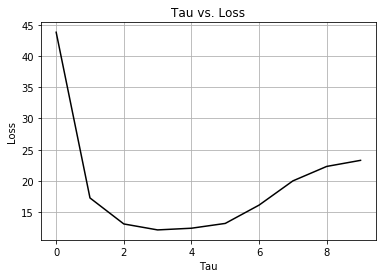
\includegraphics[scale=1.0]{10TauMean.png}

For $\tau = 200$:

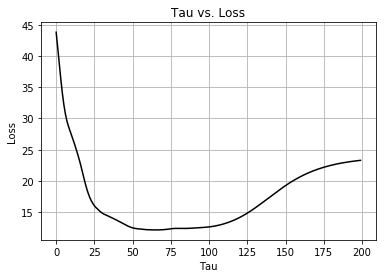
\includegraphics[scale=1.0]{200TauMean.png}

\pagebreak
For $\tau = 1000$:

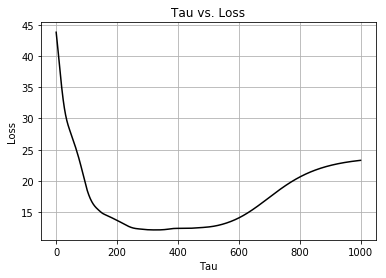
\includegraphics[scale=1.0]{1000TauMean.png}

\subsection{(4) Algorithm Behaviour for $\tau \to 0$ and $\tau \to \infty$}

From the graphs in the \hyperref[sec:kfold]{previous section}, we note that as \textbf{$\tau$ approaches 0}, it \textbf{increases drastically} in value and \textbf{approaches a value of 44}.
\\ \\
Similarly, from the graphs in the \hyperref[sec:kfold]{previous section}, we note that as \textbf{$\tau$ approaches $\infty$}, the \textbf{value stabilizes }to \textbf{approximately 24}.


\section{(Part 3) Mini-batch SGD Gradient Estimator}

\subsection{(1) Mini-Batch Proof}
\label{sec:mbp}
We need to prove that: 

\[
\mathbb{E}_{I}[
\frac{1}{m}
\sum_{i \epsilon I}a_{i}]
=
\frac{1}{n}
\sum_{i = I}^{n}a_{i}
\]

The expected value of a given variable can be expanded to: 

\[
\mathbb{E}[X]
=
\sum_{x}^{S}
p(x)f(x)
\]

where $p(x)$ is the probability function of x and $f(x)$ is the given value of x over the entire sample space $S$.

Applying this identity on the L.H.S of the first equation, we get:

\[
\mathbb{E}_{I}[
\frac{1}{m}
\sum_{i \epsilon I}a_{i}]
=
\sum_{I}p(I)
(
\frac{1}{m}
\sum_{i \epsilon I}a_{i}
)
\]

\[
=
\frac{1}{m}
\sum_{I}p(I)
(
\sum_{i \epsilon I}a_{i}
)
\]

As $p(I)$ is uniformly distributed equally and we take $\binom{n}{m}$ such batches, the equation can be rewritten as: 

\[
=
\frac{1}{m \times \binom{n}{m}}
\sum_{j = 1}^{\binom{n}{m}}
\sum_{i \epsilon I_{j}}a_{i}
\]

Expanding the $\binom{n}{m}$, we get: 

\[
=
\frac{m! (n-m)!}{m \times n!}
\sum_{j = 1}^{\binom{n}{m}}
\sum_{i \epsilon I_{j}}a_{i}
\]

This simplifies to: 

\[
=
\frac{(m-1)! (n-m)!}{n!}
\sum_{j = 1}^{\binom{n}{m}}
\sum_{i \epsilon I_{j}}a_{i}
\]

The $\sum\sum$ represents all sum of all entries in a min-batch, for all min-batches. Therefore it can be written as the sum of all mini-batches:

\[
=
\frac{(m-1)! (n-m)!}{n!}
\sum_{i = 1}^{n} 
\binom{n-1}{m-1}
a_{i}
\]

The binomial constants can be taken out and expanded to: 

\[
=
\frac{(m-1)! (n-m)!}{n!}
\times
\frac{(n-1)!}{(m-1)!(n-m)!}
\sum_{i = 1}^{n} 
a_{i}
\]

This results in the final answer of: 

\[
\mathbb{E}_{I}[
\frac{1}{m}
\sum_{i \epsilon I}a_{i}]
=
\frac{1}{n}
\sum_{i = I}^{n}a_{i}
\]

Thus proved.

\subsection{(2) Show $\mathbb{E}_{I}[\nabla L_{I}(x,y,\theta)] = \nabla L(x,y,\theta)$}

\textbf{The solution is:}

From the instructions, take: 

\[
L_{I}(x,y,\theta) = 
\frac{1}{m}
\sum_{i \epsilon I}
l(\textbf{x}^{(i)},y^{(i)},\theta)
\]

Apply the gradient on both sides:

\[
\nabla L_{I}(x,y,\theta) = 
\frac{1}{m}
\sum_{i \epsilon I}
\nabla l(\textbf{x}^{(i)},y^{(i)},\theta)
\]

Apply the Expected value on both sides: 

\[
\mathbb{E}_{I}[
\nabla L_{I}(x,y,\theta)] = 
\frac{1}{m}
\sum_{i \epsilon I}
\mathbb{E}_{I}[\nabla l(\textbf{x}^{(i)},y^{(i)},\theta)]
\]

Both $\mathbb{E}_{I}$ and $\nabla$ are linear operators that can be exchanged \textbf{if} the function is sufficiently smooth and bounded (which the loss function is). Therefore, over a uniform dataset, $U$, we can rewrite: 

The identity: 
\[
\mathbb{E}_{n\sim U}[\nabla L_n(w)] 
= \nabla\ \mathbb{E}_{n\sim U}[ L_n(w)] 
\]

First, we take the the expected value and the gradient outside the summation: 
\[
\mathbb{E}_{I}[
\nabla L_{I}(x,y,\theta)] = 
\mathbb{E}_{I}[
\nabla(
\frac{1}{m}
\sum_{i \epsilon I}
l(\textbf{x}^{(i)},y^{(i)},\theta)])
\]

Applying the identity, we can switch the $\nabla$ and the $\mathbb{E}_{I}$:

\[
\mathbb{E}_{I}[
\nabla L_{I}(x,y,\theta)] = 
\nabla
\color{purple}{(
\mathbb{E}_{I}[
\frac{1}{m}
\sum_{i \epsilon I}
l(\textbf{x}^{(i)},y^{(i)},\theta)])}
\]

From the \hyperref[sec:mbp]{previous question}, we get the following statement (which we had to prove): 

\[
\mathbb{E}_{I}[
\frac{1}{m}
\sum_{i \epsilon I}
a_{i}]= 
\frac{1}{n}
\sum_{i =1}^{n}
a_{i} 
\]

Applying the statement to the current equation and substituting the \color{purple}{purple part}\color{black}, we get this: 

\[
\mathbb{E}_{I}[
\nabla L_{I}(x,y,\theta)] = 
\nabla
{(
\frac{1}{n}
\sum_{i =1}^{n}
l(\textbf{x}^{(i)},y^{(i)},\theta)])}
\]

Which is basically: 

\[
\mathbb{E}_{I}[
\nabla L_{I}(x,y,\theta)] = 
\nabla(
L(\textbf{x},y,\theta))
\]

Thus proved.

\subsection{(3) Importance of the Previous Result}

In simple English, the previous part asked us to show that the gradient of a mini-batch is a good estimator (equal to) for the gradient of the entire Loss function. 
\\ \\ 
It is important as it \textbf{mathematically justifies sampling and the use of the mini-batch's gradient as an estimator of the gradient of the entire data set}.

\subsection{(4a) $\nabla L$ for Cost Function}

Given that: 

\[
L(x,y,\theta) = 
\frac{1}{n}
\sum_{i =1}^{n}
l(\textbf{x}^{(i)},y^{(i)},\theta))
\]

and the loss function $l(\textbf{x}^{(i)},y^{(i)},\theta)$ is: 

\[
l(\textbf{x}^{(i)},y^{(i)},\theta)) = 
(y - w^{T}\textbf{x})^{2}
\]

Therefore, 

\[
L(x,y,\theta) = 
\frac{1}{n}
\sum_{i =1}^{n}
(y - w^{T}\textbf{x})^{2}
\]

Transforming the equations into vectors and matrices in the same manner as was done in class and in the  \hyperref[sec:lsp]{Solution to the Weighted Least Square Problem} earlier.
\\ \\
Therefore, the equation can be represented as: 
\[
L(x,y,w) = 
\frac{1}{n}
||\textbf{y} - \textbf{Xw}||^{2}
\]

Applying the exact same steps as performed in the \hyperref[sec:lsp]{Solution to the Weighted Least Square Problem}, we get: 

\[ 
L(x,y,w) = 
\frac{1}{n} 
(\textbf{y}^T\textbf{y}
- 2\textbf{w}^T\textbf{X}^T\textbf{y}
+ \textbf{w}^T\textbf{X}^T\textbf{X}\textbf{w}
)
\]

This differentiates to (w.r.t $w$):

\[
\nabla(L(\textbf{w})) = 
\frac{2}{n} 
(
\textbf{X}^T\textbf{X}\textbf{w}
-\textbf{X}^T\textbf{y}
)
\]

Thus solved.

\subsection{(5) True Gradient ($\nabla L$)vs. Batch Gradient Comparisons}

The weights obtained from the true gradient, $\nabla L$ have been compared with the weights obtained by performing batch gradients using the following metrics: 

\begin{itemize}
\item \textbf{Squared Distance Metric} gives a value of 825.083. The larger the values, the larger the difference in their magnitudes.
\item \textbf{Cosine Similarity} gives a value of 0.999999942522, where 1 is for identical vectors.
\end{itemize}

\textbf{It would be more meaningful to take the cosine similarity metric} in this case. Differences in the magnitudes between the batch gradient and true gradient weights can be high. However, the weight signifies the importance of a parameter relative to other parameters. The cosine similarity check compares that and therefore, it is more meaningful.

\pagebreak
\subsection{(6) Plot $\log{\sigma_{  ̃j}}$ against $\log m$}

The single parameter chosen,  $w_{j}$ was the RM (average number of rooms per dwelling) for $j=5$ and the graph was plotted for $m$ in the range of [0,400] and $K = 500$: 

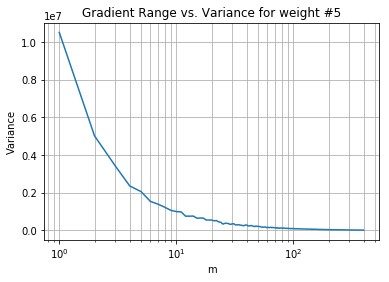
\includegraphics[scale=1]{plot1.png}
\fi